
%% bare_jrnl.tex
%% V1.4b
%% 2015/08/26
%% by Michael Shell
%% see http://www.michaelshell.org/
%% for current contact information.
%%
%% This is a skeleton file demonstrating the use of IEEEtran.cls
%% (requires IEEEtran.cls version 1.8b or later) with an IEEE
%% journal paper.
%%
%% Support sites:
%% http://www.michaelshell.org/tex/ieeetran/
%% http://www.ctan.org/pkg/ieeetran
%% and
%% http://www.ieee.org/

%%*************************************************************************
%% Legal Notice:
%% This code is offered as-is without any warranty either expressed or
%% implied; without even the implied warranty of MERCHANTABILITY or/Users/biwenwang/Desktop/Screen Shot 2019-06-13 at 1.48.20 PM.png
%% FITNESS FOR A PARTICULAR PURPOSE! 
%% User assumes all risk.
%% In no event shall the IEEE or any contributor to this code be liable for
%% any damages or losses, including, but not limited to, incidental,
%% consequential, or any other damages, resulting from the use or misuse
%% of any information contained here.
%%
%% All comments are the opinions of their respective authors and are not
%% necessarily endorsed by the IEEE.
%%
%% This work is distributed under the LaTeX Project Public License (LPPL)
%% ( http://www.latex-project.org/ ) version 1.3, and may be freely used,
%% distributed and modified. A copy of the LPPL, version 1.3, is included
%% in the base LaTeX documentation of all distributions of LaTeX released
%% 2003/12/01 or later.
%% Retain all contribution notices and credits.
%% ** Modified files should be clearly indicated as such, including  **
%% ** renaming them and changing author support contact information. **
%%*************************************************************************


% *** Authors should verify (and, if needed, correct) their LaTeX system  ***
% *** with the testflow diagnostic prior to trusting their LaTeX platform ***
% *** with production work. The IEEE's font choices and paper sizes can   ***
% *** trigger bugs that do not appear when using other class files.       ***                          ***
% The testflow support page is at:
% http://www.michaelshell.org/tex/testflow/



\documentclass[journal]{IEEEtran}
\usepackage{cite}
\usepackage[pdftex]{graphicx}
\usepackage{amsmath}
\usepackage{algorithmic}
\usepackage{array}
\usepackage{caption}
\usepackage{multirow}
\usepackage[linesnumbered,ruled,vlined]{algorithm2e} 
\setlength{\textfloatsep}{5pt}
\usepackage{stfloats}
\usepackage{amssymb}
\usepackage{pgfplots}
\usepackage{tikz}


\hyphenation{op-tical net-works semi-conduc-tor}
\begin{document}
\title{Automatic Tracking of Guidewire Tip From Fluoroscopic Videos Using RuSio Framework}


\author{Cheng Wang, Biwen Wang, Chichi Li
\thanks{Cheng Wang, Biwen Wang and Chichi Li are with Shenzhen Institutes of Advanced Technology Chinese Academy of Sciences ,China}
\thanks{Biwen Wang with Fordham University, NY, xxxxx USA}
\thanks{Manuscript received April 19, 2005; revised August 26, 2015.}}


\markboth{Journal of \LaTeX\ Class Files,~Vol.~14, No.~8, August~2015}
{Shell \MakeLowercase{\textit{et al.}}: Bare Demo of IEEEtran.cls for IEEE Journals}


\maketitle


\begin{abstract}
In modern cardiovascular intervention surgery, guidewire serves as a trailblazer to guide the movement of the micro-catheter or catheter. The distal of the guidewire can be considered as a random curvilinear structure, and the tip of the guidewire can measure some required parameters. Computer-assisted intervention could enhance the system's automation level and reduce interventionists' fatigue caused by tracking the guidewire tip on the fluoroscopic screen. Therefore, the development of detecting and analyzing the guidewire tip in real-time practice becomes imperative. The purpose of this paper is to propose RuSio, a random curvilinear structure's morphological feature-based motion tracking framework, which provides real-time and accurate information of the guidewire tip. Compared to prior works, our framework contains a set of approaches to eliminate non-guidewire tip objects and depict the shape of guidewire tip during the tracking process while no previously model built up or pre-operative vascular morphology references needed. RuSio framework achieves on average above 90\% accuracy for tracking the curvilinear structure with latency less than 700ms among 8 experiments conducted. Also, RuSio could distinguish the guidewire tip from other curvilinear structures under low doses X-ray circumstance. This algorithm has been implemented into the software.
\end{abstract}


\begin{IEEEkeywords}
computer-assisted surgery, real-time tracking, curvilinear structure
\end{IEEEkeywords}

\IEEEpeerreviewmaketitle



\section{Introduction}
\IEEEPARstart{C}{ompare}
to conventional surgery, endovascular intervention surgery minimize invasiveness and reduce patients' recovery time. Guidewire, a tool that could insert into the vessel through a catheter, makes a great contribution for monitoring and assisting intervention. A great application is that during cardiovascular intervention process, the guidewire is inside of the catheter, and they move alternatively towards the lesion inside the coronary branches. With the rapid development of the computer-assisted intervention, increasing numbers of algorithms have been applied to make the clinical process intelligent. Therefore, it is crucial to have a robust tracking system that provides reliable guidewire, also guidewire tip's locations and shapes in the form of consecutive images. Moreover, the movement of the guidewire tip offers some important information such as can be used to evaluate a doctor's intervention technique. Two sequences are superimposed for the following time series(Fig.1) using the stack composition technology of Photoshop. Additional consensus is reach by collecting data from all recorded videos that the motion of guidewire tip is affected by factors such as breathing and heartbeats.

\begin{figure}[!hbtp] 
	\centering
	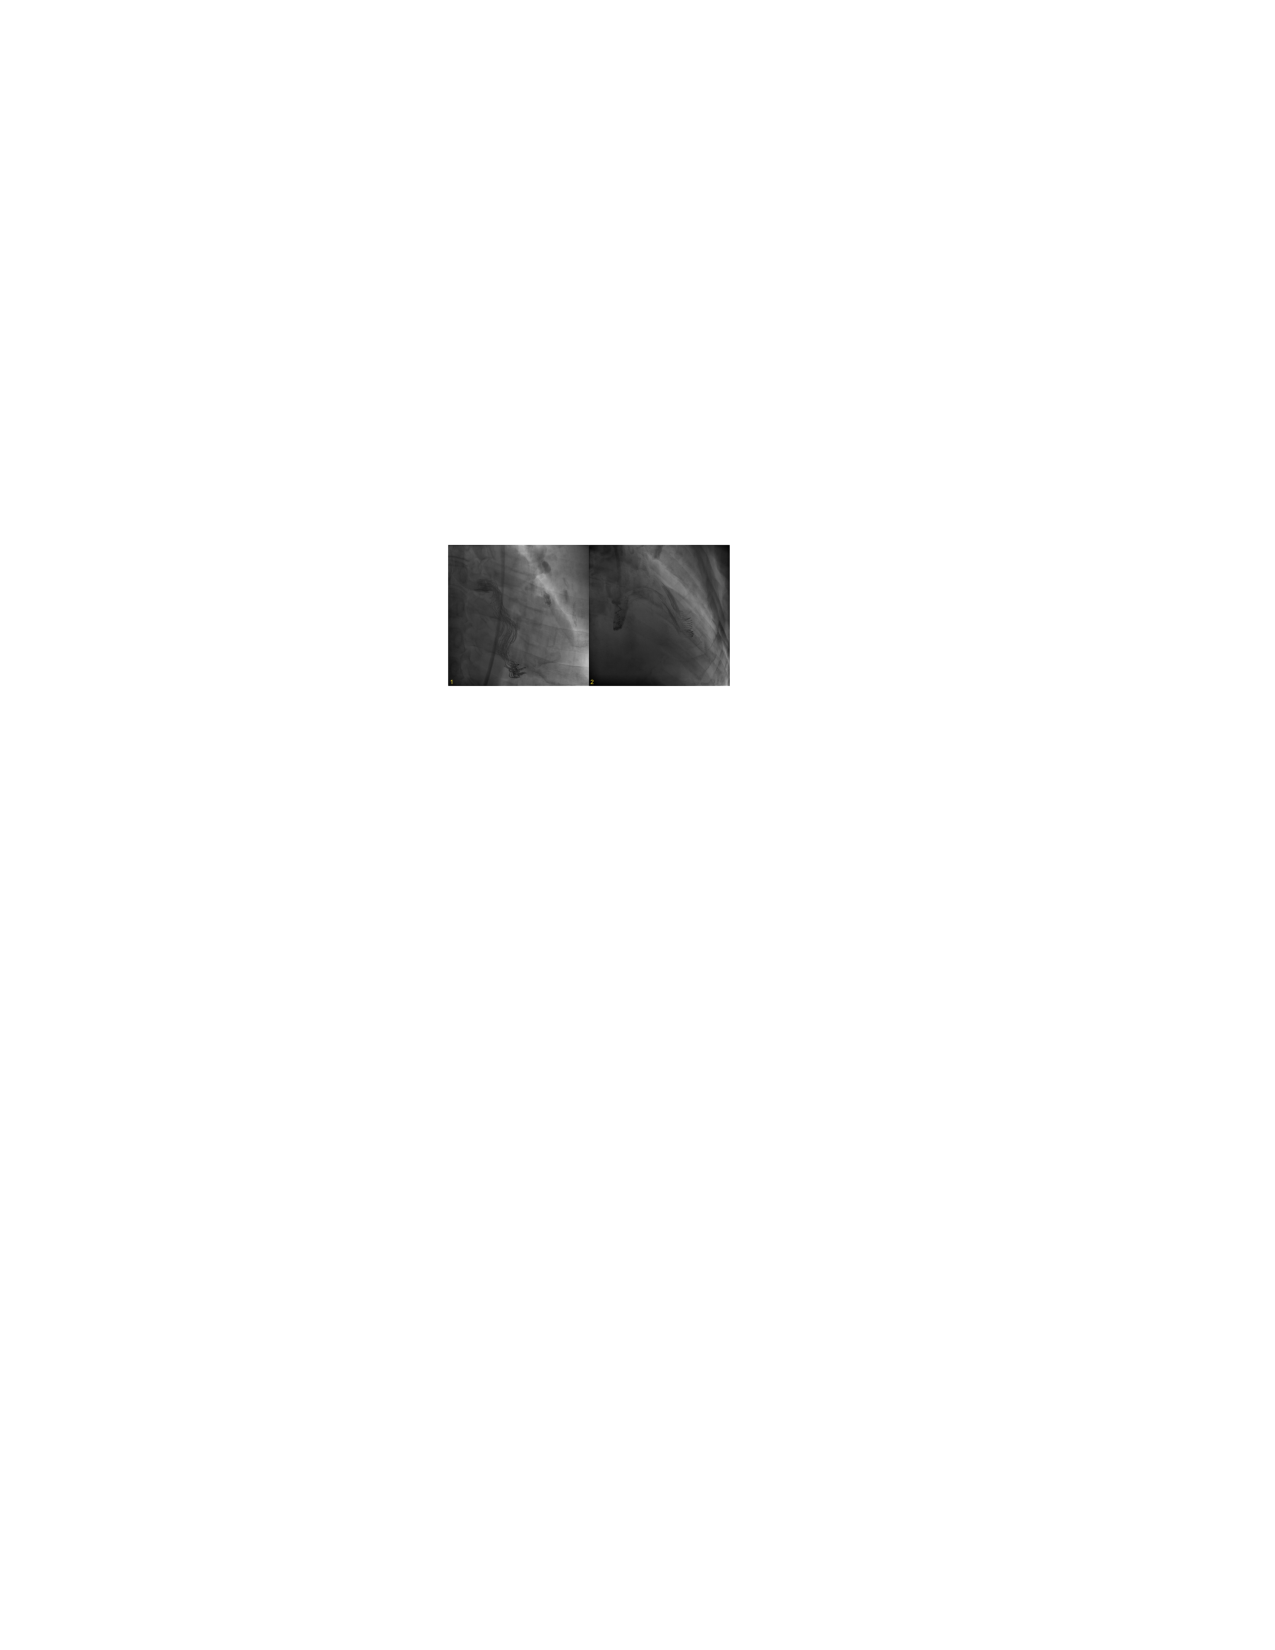
\includegraphics[width=3.5in]{figures/figure1}
		\caption{1.The relative position of catheter and its containing guidewire tip changes irregularly, which increases the tracking difficulty. 2.The motion direction of the guidewire tip is approximately overlap with the rib. } 
	\label{fig:mcmthesis-logo} 
\end{figure}

Currently, lots of traditional tracking algorithms have been proposed. KCF(Kernelized Correlation Filters) \cite{Henriques2014High} which combined ridge regression with cyclically shifted to achieve 73.8\% precision and 172 FPS in 50 videos. GOTURN(Generic Object Tracking Using Regression Networks)\cite{held2016learning} is a novel method that uses Neural Network and trained offline, which can track a novel object at 100FPS. Most traditional tracking algorithms can reach a satisfying level of tracking moving objects. However, objects tracked by traditional tracking method have high Singal-Noise ratio compared to guidewire tip in fluoroscopy videos which imposes problems. Therefore, several algorithms have been proposed for tracking or segmenting of the guidewire. To this state, most guidewire tracking algorithms are based on Bayesian framework that uses sequential data to predict unknown states \cite{Isard1998}.
In \cite{bacchuwar2017voidd}, it suggests the centerline of vessel and ECG information can be served as references during tracking of the guidewire tip. 
In \cite{Peng2009Hierarchical}, Hierarchical guidewire tracking has been proposed using the rigid motion of guidewire between two frames with each frame less than 1s, and the guidewire body tracking precision is less than 0.18mm, but in fluoroscopic videos the guidewire tip is non-rigid. Wang et al. \cite{wang2017guide} presented an approach based on edge detection and open active contours with 95.3\% accuracy. However, the method focuses on a single frame, and it takes about 3.79s to process each frame. Recently Ma et al. \cite{ma2018novel} proposed a framework which can detect multiple catheters or guidewires at the same time; however, the process of eliminating other curvilinear objects is not satisfiable during the tracking. To solve the problem that targets will be lost if large movement occurs between two consecutive frames, segment-like features(SEGlets) is introduced to deal with the problem in\cite{vandini2017robust}.

Different from related works, our tracking approach uses the information from original X-ray fluoroscopic videos to provide reliable information of guidewire tip without using external references. Moreover, the framework can distinguish the guidewire tip from candidates based on their motion information in time series without parameter configuration in advance. The main contribution of our work is to propose RuSio(Random Curvilinear Structure's Morphological Feature-Based Motion Tracking) framework which includes a novel single non-rigid curvilinear structure target tracking strategy and a sophisticated procedure to achieve automatic recognition of the guidewire tip in fluoroscopic video. The framework has been designed and implemented by our research team, using python, in the open source software which is available on https://github.com/\footnote{The detailed url can be provided after review process}. 9 fluoroscopic videos under the scenarios of cardiovascular intervention, provided by Zhong Da Hospital Southeast University and Peking Union Medical College Hospital, have been validated and shown promising performance. 


\section{Methods}
Real-time guidewire tip tracking process is a crucial element in cardiovascular intervention procedure. Furthermore, It's hard to distinguish the guidewire tip and other curvilinear structures in some exceptional circumstances. Clinical data presented information from many perspectives gives insight for solving the problems mentioned above. The guidewire is a curvilinear structure which is distinguishable compared with other guidewire-like structures since the movement of guidewire-like structures is dissimilar. For example, the movement of the rib is static while as the movement of catheters in blood vessels is periodic. Therefore, non-guidewire tip structures could be eliminated based on these features. Additionally, a sophisticate multi-guidewire-like feature points extracting and tracking algorithm has been proposed. The algorithm will mark and track all potential curvilinear structures. Furthermore, non-guidewire tip area will be rapidly eliminated in a tolerant time interval which is usually less than 36 frames(3 seconds). This framework has been validated on 9 fluoroscopic videos under the scenarios of cardiovascular intervention. Two novel ideas have been proposed in the algorithm: (a) A restricted area which called predicted guidewire tip area(PGA) has been used during tracking to enhance tracking efficiency and accuracy. (b) The framework solved segments disconnection and eliminated noises during extraction and segmentation of the guidewire tip.
\par
Each component of RuSio framework will be described in details in the following sections. The detection of guidewire tip feature is shown in Sec A, guidewire tip prediction is described in Sec.B, detailed explanation of tracking a single target region is in Sec.C. Finally, the decision making principle which builds in RuSio framework is shown in Sec.D. The complete pseudo code of RuSio framework is shown at the end of Method.

\begin{figure}[!htb]
	\centering  
	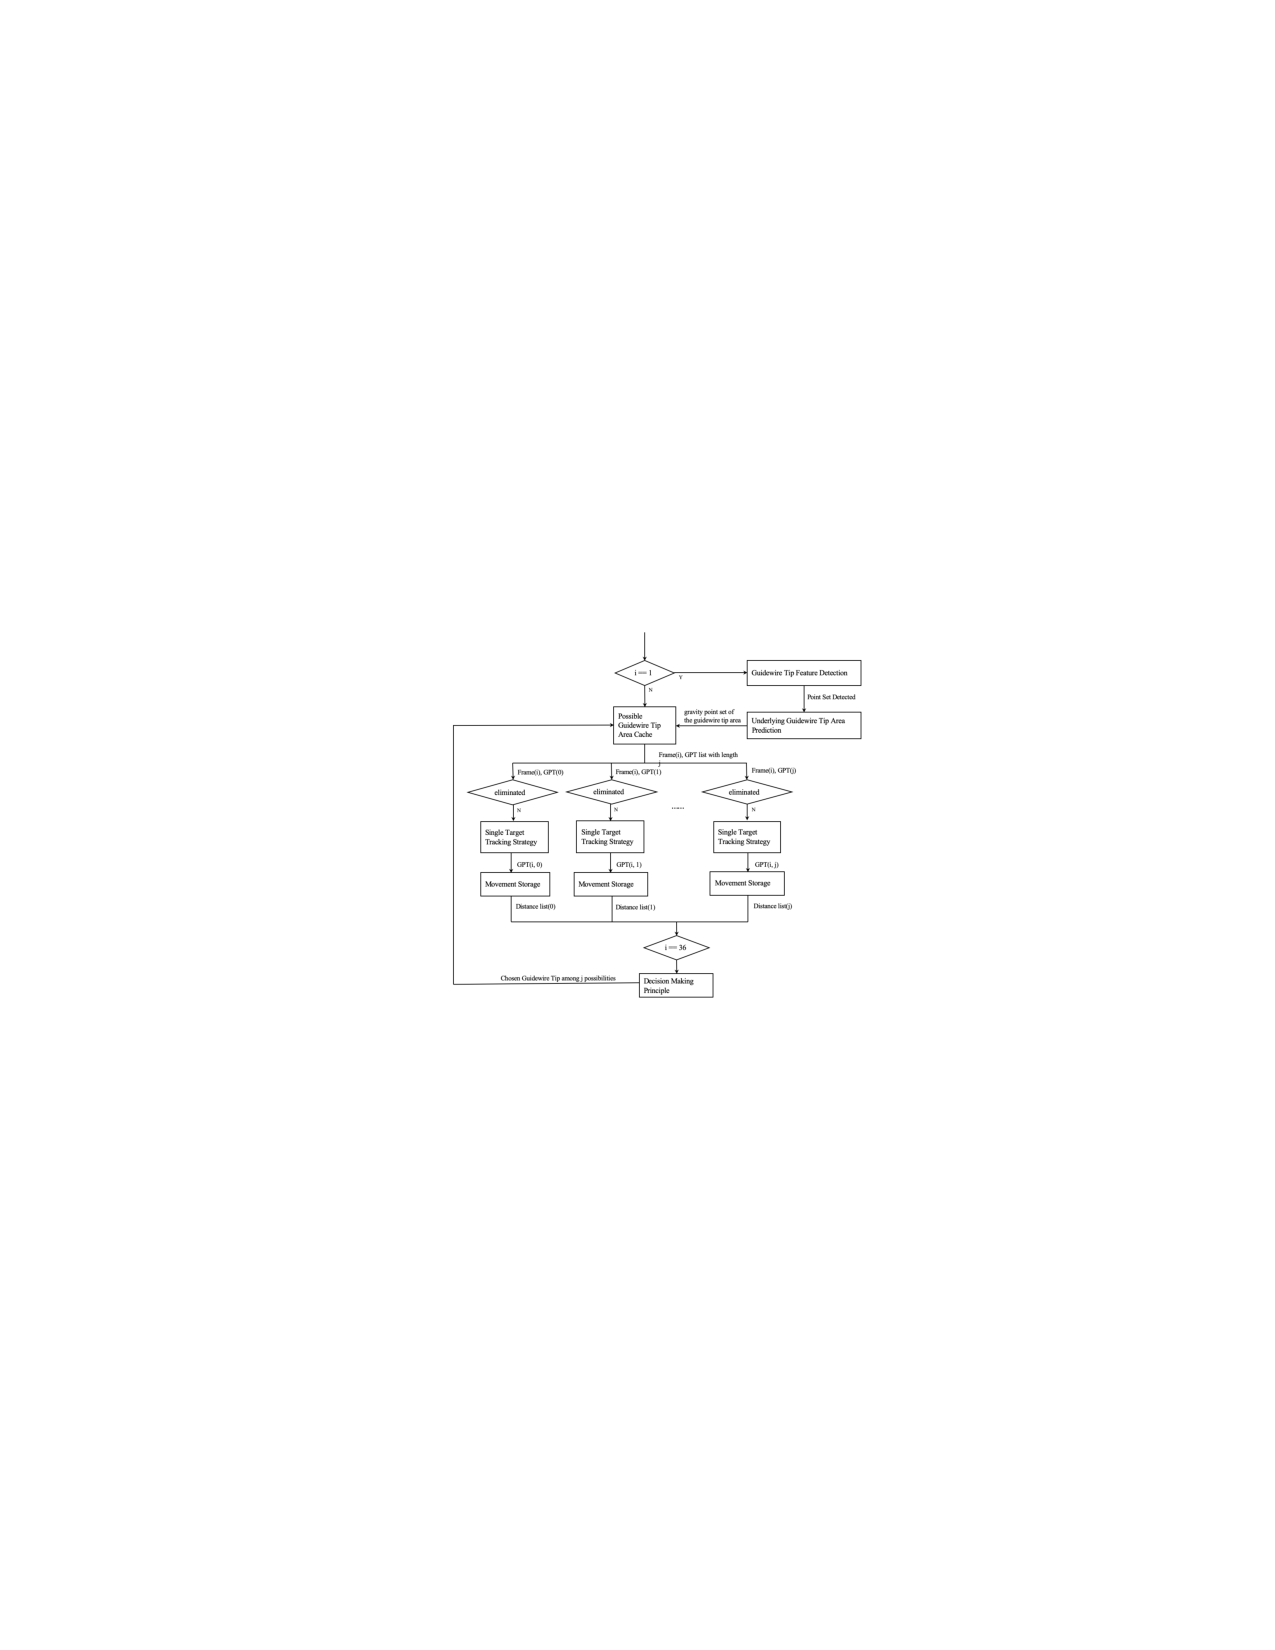
\includegraphics[width=3.5in]{figures/figure2}
		\caption{RuSio framework flowchart} 
	\label{fig:mcmthesis-logo} 
\end{figure}



\subsection{Guidewire Tip Feature Detection(GTFD)}
As it is mentioned above, detecting the locations of underlying guidewire tips plays a fundamental role in the tracking process. Frangi's multi-scale vessel enhancement\cite{frangi1998multiscale} combined with Gradient Vector Flow(GVF), introduced by Bauer et al. \cite{bauer2008novel}, which detects tubular structures are used during guidewire tip feature detection. This detection method is mainly divided into two parts: curvilinear structure enhancement and feature points extraction.
\subsubsection{Enhancement} 
A curvilinear structure enhancement procedure is used to improve intensity projection display, which will enhance the tubular structure's delineation. After enhancement, the guidewire tip can be highlighted from the cardiovascular image since the guidewire tip is a curvilinear structure which also has tubular features.
In 1998, Frangi et al. \cite{frangi1998multiscale} implemented vessel enhancement filter based on multiple scales. However, the characteristic of guidewire tip such as length, width is fixed. Therefore, a single scale can be used here to reduce the computational workload and to extract guidewire tip among multiple scales of tubular objects.
Let $I(x,y)$ be an image, the Hessian matrix of the image $H(x,y)$ is:
\begin{equation}
H(x,y)= 
\left[\begin{array}{ccc}
I_{xx}(x,y) & I_{xy}(x,y)\\
I_{xy}(x,y) & I_{xy}(x,y)
\end{array}
\right]
\end{equation}
In this paper, $\lambda1$ and $\lambda2$ are two smallest eigenvalues of Hessian matrix and $|\lambda_1|$ $<$ $|\lambda_2|$. The guidewire tip structure enhancement function is defined as:
\begin{equation}
F=\left\{
\begin{array}{ccc}
0 & &  {if \lambda_2 > 0}\\
e^{\frac{-R^{2}_B}{2 \beta}}(1-e^{\frac{-S^{2}}{2\gamma^{2}}}) & & {otherwise}
\end{array} \right.
\end{equation}

$\beta$ and $\gamma$ are thresholds that control the sensitivity of the filter. For 2D image, $R_B$ is used to distinguish curvilinear structure:
\begin{equation}{
R_B = \frac{\lambda_1}{\lambda_2}}
\end{equation}
and 
\begin{equation}{ 
S = \sqrt{\lambda_1^{2}+ \lambda_2^{2}}}
\end{equation}
is used to eliminate the regions that the image intensity variations are small.
\subsubsection{Feature Points Extraction}
Gradient Vector Flow(GVF) field is defined as a new class of external force field $F_{ext} = V(x,y)$. With a suitable scale, the gradient information points to the center of the tubular object, which means guidewire tip and other tubular structures can be extracted.
By spreading out the gradient vector on the image, GVF field can enlarge the capture range and progress into boundary concavities. Let $f(x,y)$ be the edge map and $\nabla$$f(x,y)$ be the gradient edge map of image $I(x,y)$. The edge of guidewire tip has the highest value. Vector field $V(x,y)$ = [$u(x,y),v(x,y)$] is generated by iteratively diffusing the edge of image. The GVF field is defined as vector field $V(x,y)$ that minimizes:
\begin{equation}{
\epsilon = \iint \mu\nabla^{2}V+|\nabla f|^{2}|V-\nabla f|^{2} \,dx \,dy}
\end{equation}
where $\mu$ is positive regulatory factor. The value of $\mu$ depends on the quality of image. $\mu$ will be increased if the amount of noise increase. 
Let $\nabla^{2}$ be Laplacian operator. According to variational principle, GVF field can be founded by dealing with Euler equation
\begin{equation}{
\mu\nabla^{2}V+|\nabla f|^{2}|V-\nabla f|^{2}=0}
\end{equation}
Based on the direction of gradient vector on GVF field, the target points will be recorded.

\subsection{Underlying Guidewire Tip Areas Prediction(UGTAP)}
Guidewire tip structure detection provides a set of feature points which are scattered on the image. They can be separated into several clusters, but the number of clusters is unknown in advance. The underlying guidewire tips must appear in the area that the clusters are occupied. Neighbor Growing Algorithm(NGA) is used to deliver the points to corresponding clusters. The Moore Neighborhood(MN) is defined as the neighbor points which surround the central cell. With a given range $r (r \geq  1)$, the Extended Moore Neighborhood(EMN) has $(2r+1)^2-1$ cells including central cell. MN is the simplest form of EMN.
Clusters collect feature points based on searching neighborhood. If a feature point is the neighbor of any point in a cluster, it is considered that it belongs to the same cluster. On the contrary, the point pertains to a new cluster. After clustering feature points by using NGA, the gravity points of clusters are used to locate the possible guidewire tips in the first frame of the sequence. Based on the set of clusters, the image can be segmented into several parts, which is defined as target regions. The region is defined as a $m*m$ area of 2D image with gravity point as the center. From the second frame, the framework only focuses on the target region instead of the whole image. In order to get the precise location and shape of the guidewire tip, the target region needs further processing.

\begin{algorithm}[!ht]
\setlength{\abovedisplayskip}{3pt}
\setlength{\belowdisplayskip}{-3pt}
	\caption{NGA}
		\KwIn{The set of feature points $pts$\\
		The range of EMN $r$}\
		\KwOut{Cluster sets $C_n$}\
		\For{each point $pt$ in $pts$}{
			\If {pt is not included in any cluster}{
			\textbf{Put $pt$ into a new cluster $c$ and a new stack $s$}\;
			\While{$s$ is not empty}{
			\textbf{Pop point $pt'$ from $s$\;
			Construct $an$ EMN M with r around its central $pt'$}\;
				\For {each position $p$ in M}{
					\If{$p$ exits in feature points set and is not included in any cluster}{
					\textbf{Put $p$ into $c$ and $s$}\;
			
			}
				
		}
	}
}
}
\end{algorithm}


\subsection{Single Target Region Tracking Pipeline(STRT)} 

\subsubsection{Tracking Analysis}
It is challenging to track guidewire tip due to the characteristic of guidewire tip is non-rigid. However, based on a large number of clinical data observation, the range of movement and morphological change of the guidewire tip are limited between two frames in consecutive x-ray fluoroscopic images. Although the length of the guidewire tip varies as the angle of X-ray machine projection changes, the actual visible maximum length $L_{max}$ of guidewire tip will remain the same. Therefore, the tracking strategy will initiate a square patch that contains the whole configuration of the guidewire tip structure in tracking target region. 
\subsubsection{Tracking Strategy} 
Our tracking target, guidewire tip, has different Signal-Noise ratio compared to traditional tracking object such as human face which takes up a larger proportion of pixels than guidewire tip. As the morphology of guidewire tip is extracted in a current frame, the result will be used to calculate factors such as centroid, optimal square patch(OSP) that can be used to predict possible appearance region of guidewire tip in next frame. It is proven experimentally that only using OSP patch is not sufficient in tracking guidewire tip. Besides the guidewire tip, other guidewire-like structures such as ribs also lie inside of the patch, which will influence tracking accuracy and disturb curve fitting process. Therefore, an improved tracking model combined with OSP has been proposed, which called Predicted Guidewire tip Area(PGA, Fig.2), to enhance tracking accuracy and computational efficiency. Considering during intervention surgery, the manual intervention speed of surgeon is limited. Besides, the image acquisition frame rate of the X-ray machine is 7-12 FPS. Thus the movement of guidewire tip in consecutive frames will not have significant movement tendency toward the blood vessel. Therefore, the maximum move back distance(MBD) and maximum move forward distance(MFD) can be extracted. Additionally, the max amplitude affected by heartbeat and respiration is defined as MAmp. These factors(MBD, MFD and MAmp also shown in Fig.2) can be used to predict the location of guidewire in the next frame using the formula: $$PGA_{n+1} = f(GTS_{n}, \delta_{MFD}, \delta_{MBD}, Am)$$ (GTS, Guidewire Tip Structure will be described shortly.)
Benefited from our original design, PGA eliminates noise that outside the target region to make guidewire tip morphology segmentation process more focused compared with traditional tracking algorithm which only uses the bounding box.
\begin{figure}[hb]
	\centering
	\vspace{-0.2in}
	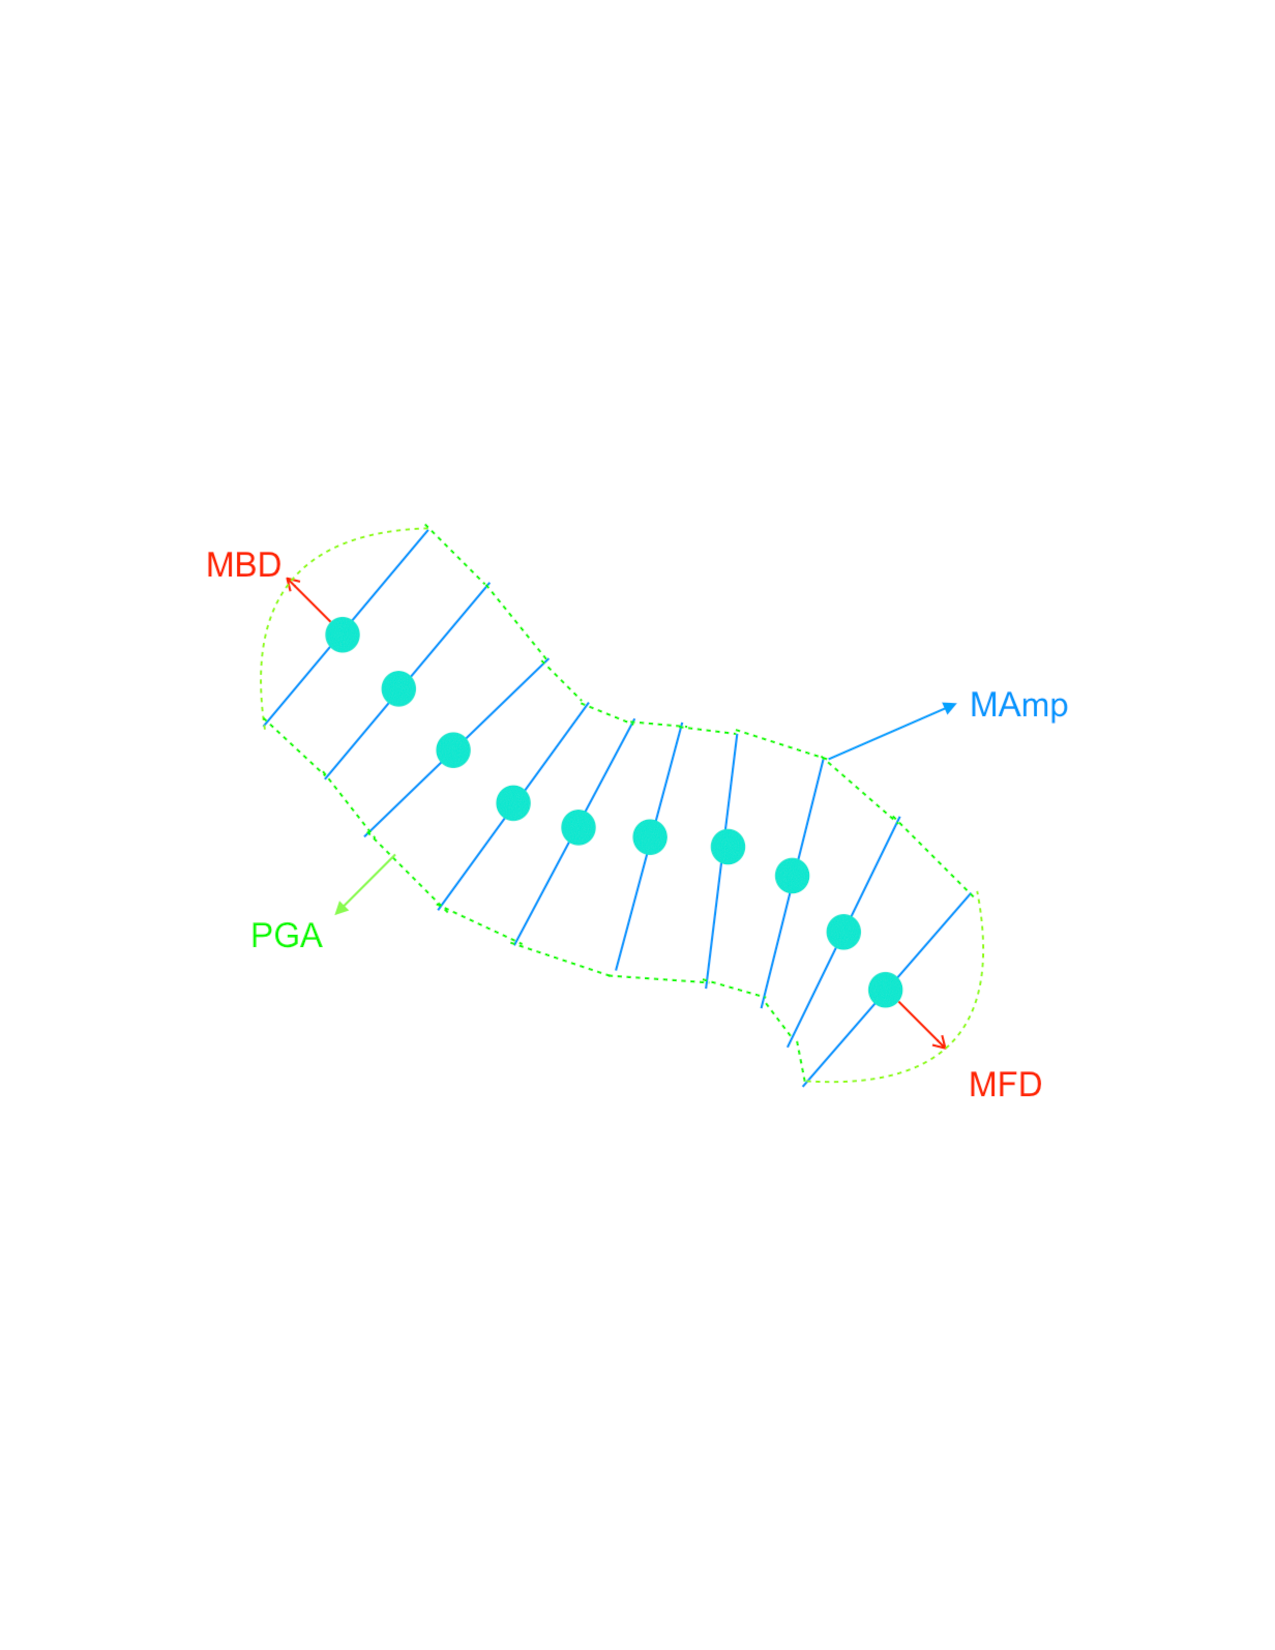
\includegraphics[width=3.5in]{figures/figure4}
	\caption{Description of Predicted Guidewire Tip Area} 
	\label{fig:mcmthesis-logo} 
\end{figure}


\begin{figure}[ht]
	\centering
	\vspace{-0.15in}
	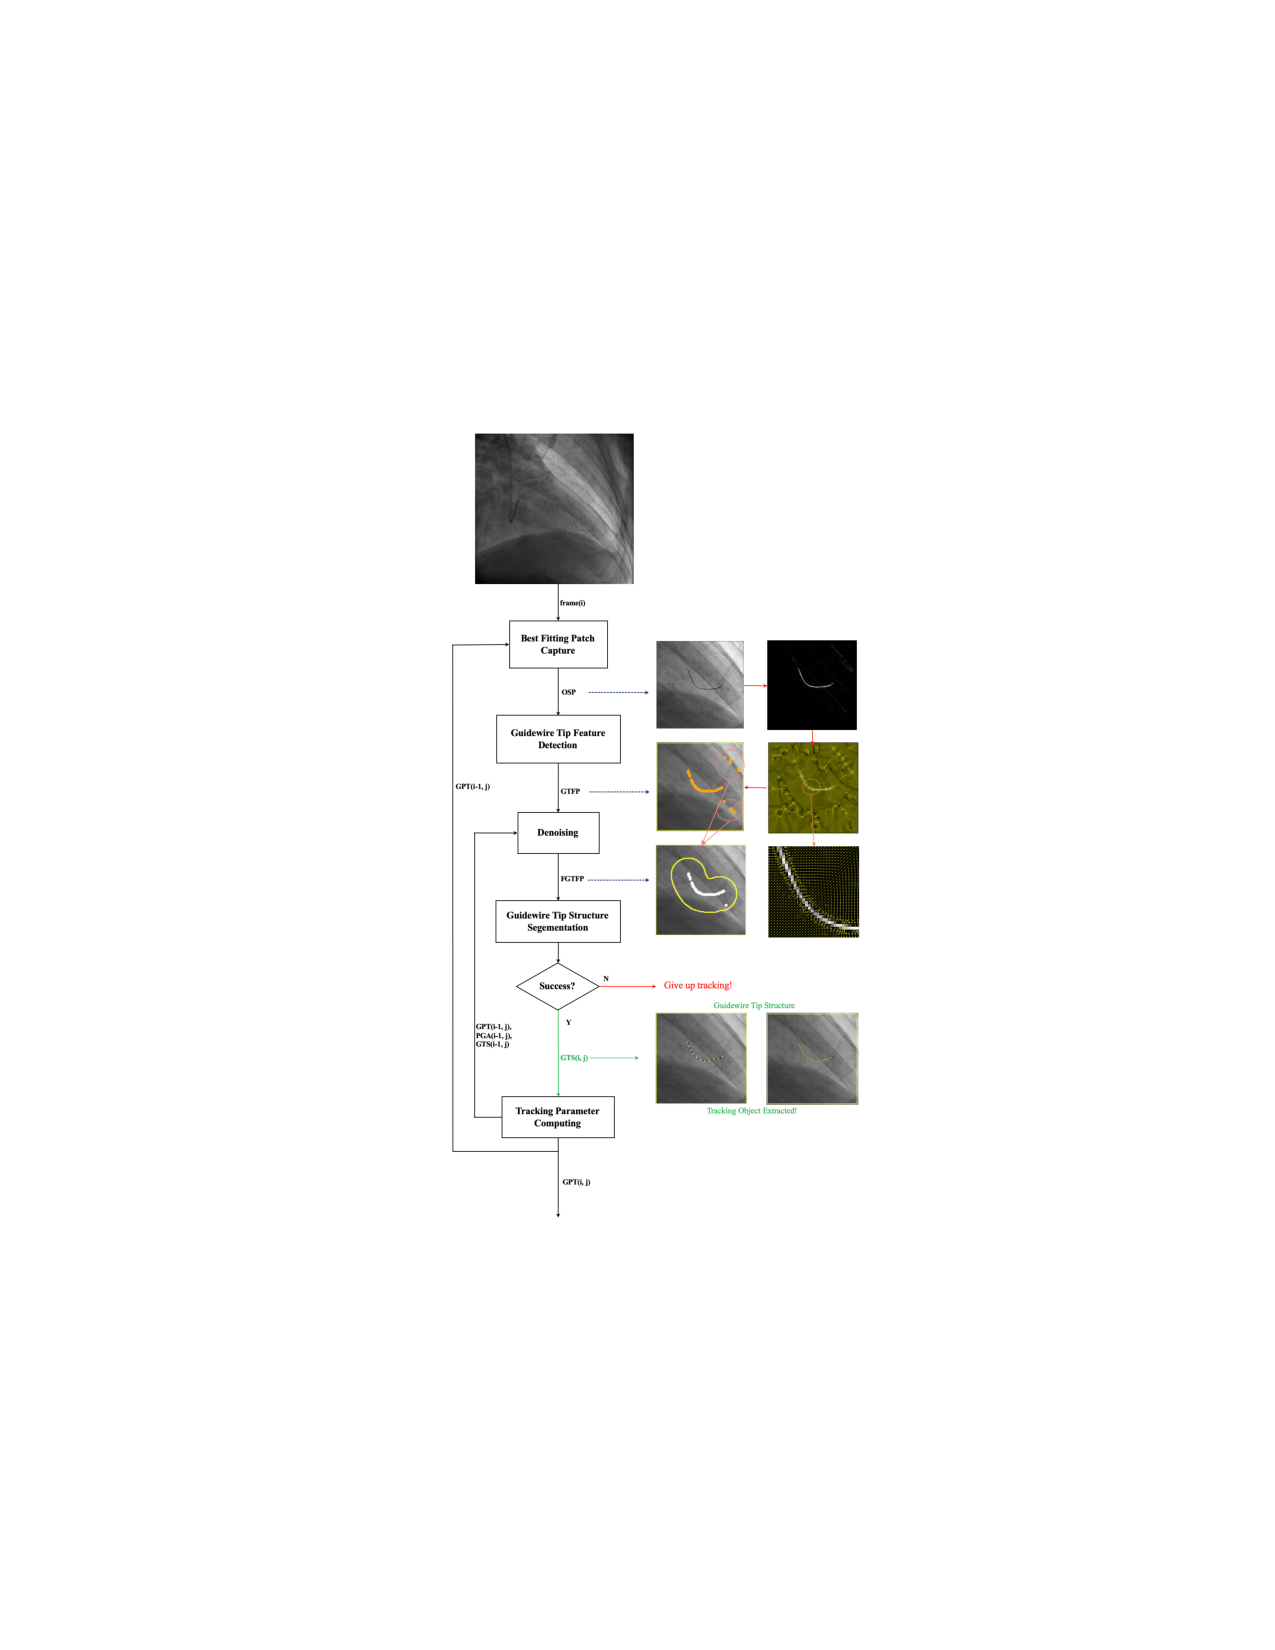
\includegraphics[width=3.5in]{figures/figure3}
		\caption{Target Region Tracking and Segmentation Pipeline Showcase where (F)GTFP is (Filtered)Guidewire Tip Feature Points} 
	\label{fig:mcmthesis-logo} 
\end{figure}

\subsubsection{Target Structure Segmentation}
As the guidewire tip feature detection procedure being applied, the feature points of guidewire tip which inside optimal square patch can be calculated. Feature points are used to calculate PGA, which already mentioned before to further eliminate noise during guidewire tip segmentation. Due to the discontinuity of some feature points, the NGA is applied in region processing with a smaller range of neighborhood, which eliminates the outliers. It may obtain several curves in one target region after filtering and extracting centerline in each cluster. However, the lengths of centerlines do not reach the minimal prediction length $l_l$ of guidewire tip in some cases. Thus, two curves are considered to be connected if both of the two conditions are satisfied: a)  The distance $d$ between the closest end points of two curves is less than a constant $D_{max}$. b) The angle $\alpha$ of two lines, which are linear regression curves based on last five adjacent points of each curve, is less than $\theta$. Based on criteria a and b, a potential guidewire tip point set is obtained. c) If the distance of those points is too far from previous frame, those points will be eliminated. Moreover, other clusters will also be eliminated in addition to satisfying above criteria. (Fig.4) Therefore, Guidewire Tip Structures(GTS) has been extracted. 


\begin{figure}[!hbtp]
	\centering 
	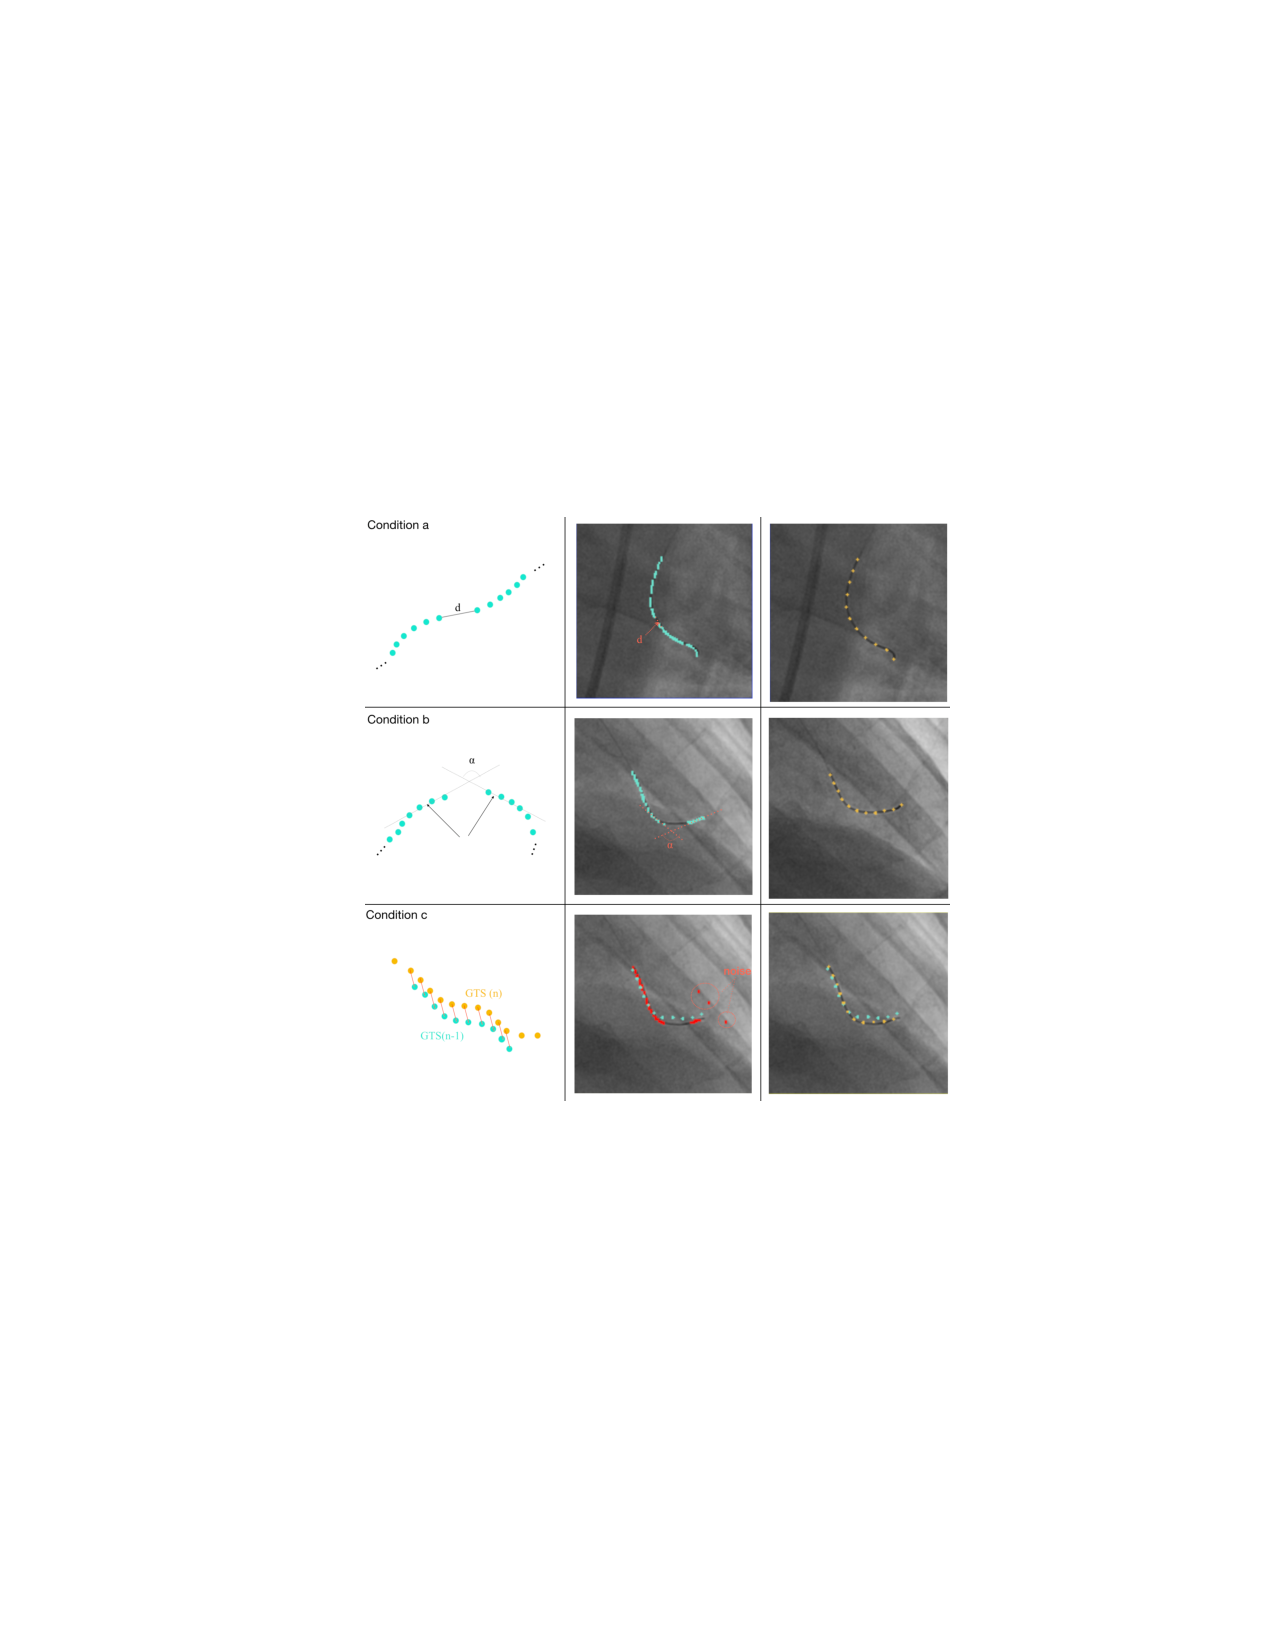
\includegraphics[width=3.5in]{figures/figure5}
		\caption{Conditions of calibration} 
	\label{fig:mcmthesis-logo} 
\end{figure}



\subsection{Decision-making Principle(DM)}
In the fluoroscopic video, plenty of moving objects have a curvilinear structure. The guidewire tip recognition procedure is a task which aims to classify different moving curvilinear objects. Under a large amount of movement tracking analysis, those curvilinear structure objects can be classified into three major categories. Firstly, static curvilinear like objects which usually occur around bones such as rib and spine. Secondly, periodic curvilinear like objects which influenced by breathing and heartbeat rate of the patients such as catheter in standby or the edge of the heart. Lastly, non-periodic curvilinear like objects which move forward or backward following with the direction of the vascular intervention can be considered as guidewire tip. 

Based on these three types of motions, it is possible to determine the guidewire tip among p candidates by using Mean Square Error(MSE). MSE calculates the average square distance differences between the gravity point(centroid) of each frame i for each candidate j and the gravity point of initial frame 0. The final decision is forced to be made in the first k sequences(k=36) using the formula: 

$$ V_{max} = \max\limits_{1<j<p} {\sum_{i=1} ^k \frac{1}{k} (d_{i,j}-d_{0,j})^2} $$
where $d_{0,j}$ is the initial frame of jth candidate and 
$$ d_{i,j} \leftarrow Edistance\Big\{gravity(GTS_{i,j}),gravity(GTS_{0,j}) \Big\}$$
$Edistance$ is Euclidean Distance.

\begin{algorithm}[!htbp]
\setlength{\abovedisplayskip}{3pt}
\setlength{\belowdisplayskip}{-3pt}
	\caption{RuSio Framework}
		\KwIn{$Img(i)$: Fluoroscopic Image i with N frames\\
		$\delta$: Final decision time time = 36 }
		\KwOut{$GTS(i)$}
		Initialise $GPT_{i,j}$ Gravity Points\; 
		Initialise $PGA_{i,j}$ Predicted Guidewire tip Area\; 
		Initialise $GTS_{i,j}$ Guidewire Tip Structures\; 
		Initialise $GPD_{i,j}$ Gravity Points Distance\; 
		Initialise $RmList$ Eliminated guidewire tip candidates\; 
		\For{$i$ = 0 $\rightarrow M-1$}{
			\If {i = 1}{
			\textbf{$pts \leftarrow$ GTFD($Img(i)$)}\;
			\textbf{$GPT_i \leftarrow$ UGTAP($pts$)}\;
			\textbf{$N \leftarrow$ len($GPT_i$)}\;
			Allocate $RmList$, $PGA_i$, $GTS_i$ with N
			}
		\For{$j$ = 0 $\rightarrow$ N-1}{
			//if current guidewire tip candidate hasn't been eliminated\\
			\If{$RmList[j]$ != 1}{
		   	\textbf{$Success$,$GPT_{i,j}$,$PGA{i,j}$,$GTS{i,j}$ $\leftarrow$ STRT($Img(i)$, $GPT_{i-1,j}$,$PGA(i-1.j)$,$GTS(i-1,j)$)}\; 
 			\textbf{$GPD_{i,j} \leftarrow$  EDistance($GPT(i,j)$,$GPT(0,j)$)}\; 
			\textbf{$OSP \leftarrow$  BondingBox($GPT(i,j)$,$80$)}\; 
		   	\If{not success}{
		   		\textbf{$RemoveList[j] \leftarrow 1$}\; 
		   	}
		   	}
		 }
		 \If{i == $\delta$}{
		 	//Return the index of most possible candidate\\
		 	\textbf{$k \leftarrow$ DM($GPD$)}\;
		 	\For{$x$ = 0 $\rightarrow$ N-1}{
		 		\If{x != k}{
		 			\textbf{$RemoveList[x]\leftarrow 1$)}\;
		 			}
		 		}
		 	}
		
		}
\end{algorithm}


\section{Experimental Validation}
In traditional tracking algorithm, bounding box over lap \cite{Henriques2014High} or precision curve \cite{Babenko2011Robust} are used to show the performance of proposed tracking algorithm. However, due to the characteristic of guidewire tip is different from traditional tracking object. We used different way to evaluate the performance of RuSio framework.The performances of RuSio framework has been recorded in both Fig.6 and Table.2. The evaluation of RuSio framework considered three parts: Recognition, Segmentation and Tracking. For segmentation accuracy evaluation, the distance between the chosen tip and ground truth is measured. If the mean distance is more than 3 pixels, the segmentation of corresponding guidewire tip is considered as failure. Also, the total frames, miss tracking rate(MTR), false tracking rate(FTR), mean discrete Frechet distance(MDF), segmentation accuracy(SA), tracking accuracy(TA) in each sequence are recorded(Table 1).
\par
Sec A recorded general information about RuSio framework implementation and dataset. The details of guidewire tip recognition and tracking performance are shown in Sec.B and Sec.C, respectively. In Section D, we shown some exceptional cases that caused low segmentation accuracy of RuSio. 


\subsection{Framework Implementation}
The evaluation of RuSio framework is conducted on 9 fluoroscopic videos from different cardiovascular intervention surgery. The use of this dataset has been approved by Peking Union Medical College Hospital and ZhongDa Hospital Southeast University. Video sequence has 1100 frames in total with a frame rate of 7FPS. The frame size of each sequence is 512*512 which pixel size is around 0.2343 mm. Our research team also designed a graphical tool to annotate the ground truth of the guidewire tip in each frame and the framework has also been implemented. 

\begin{figure}[!htb]
	\centering  
	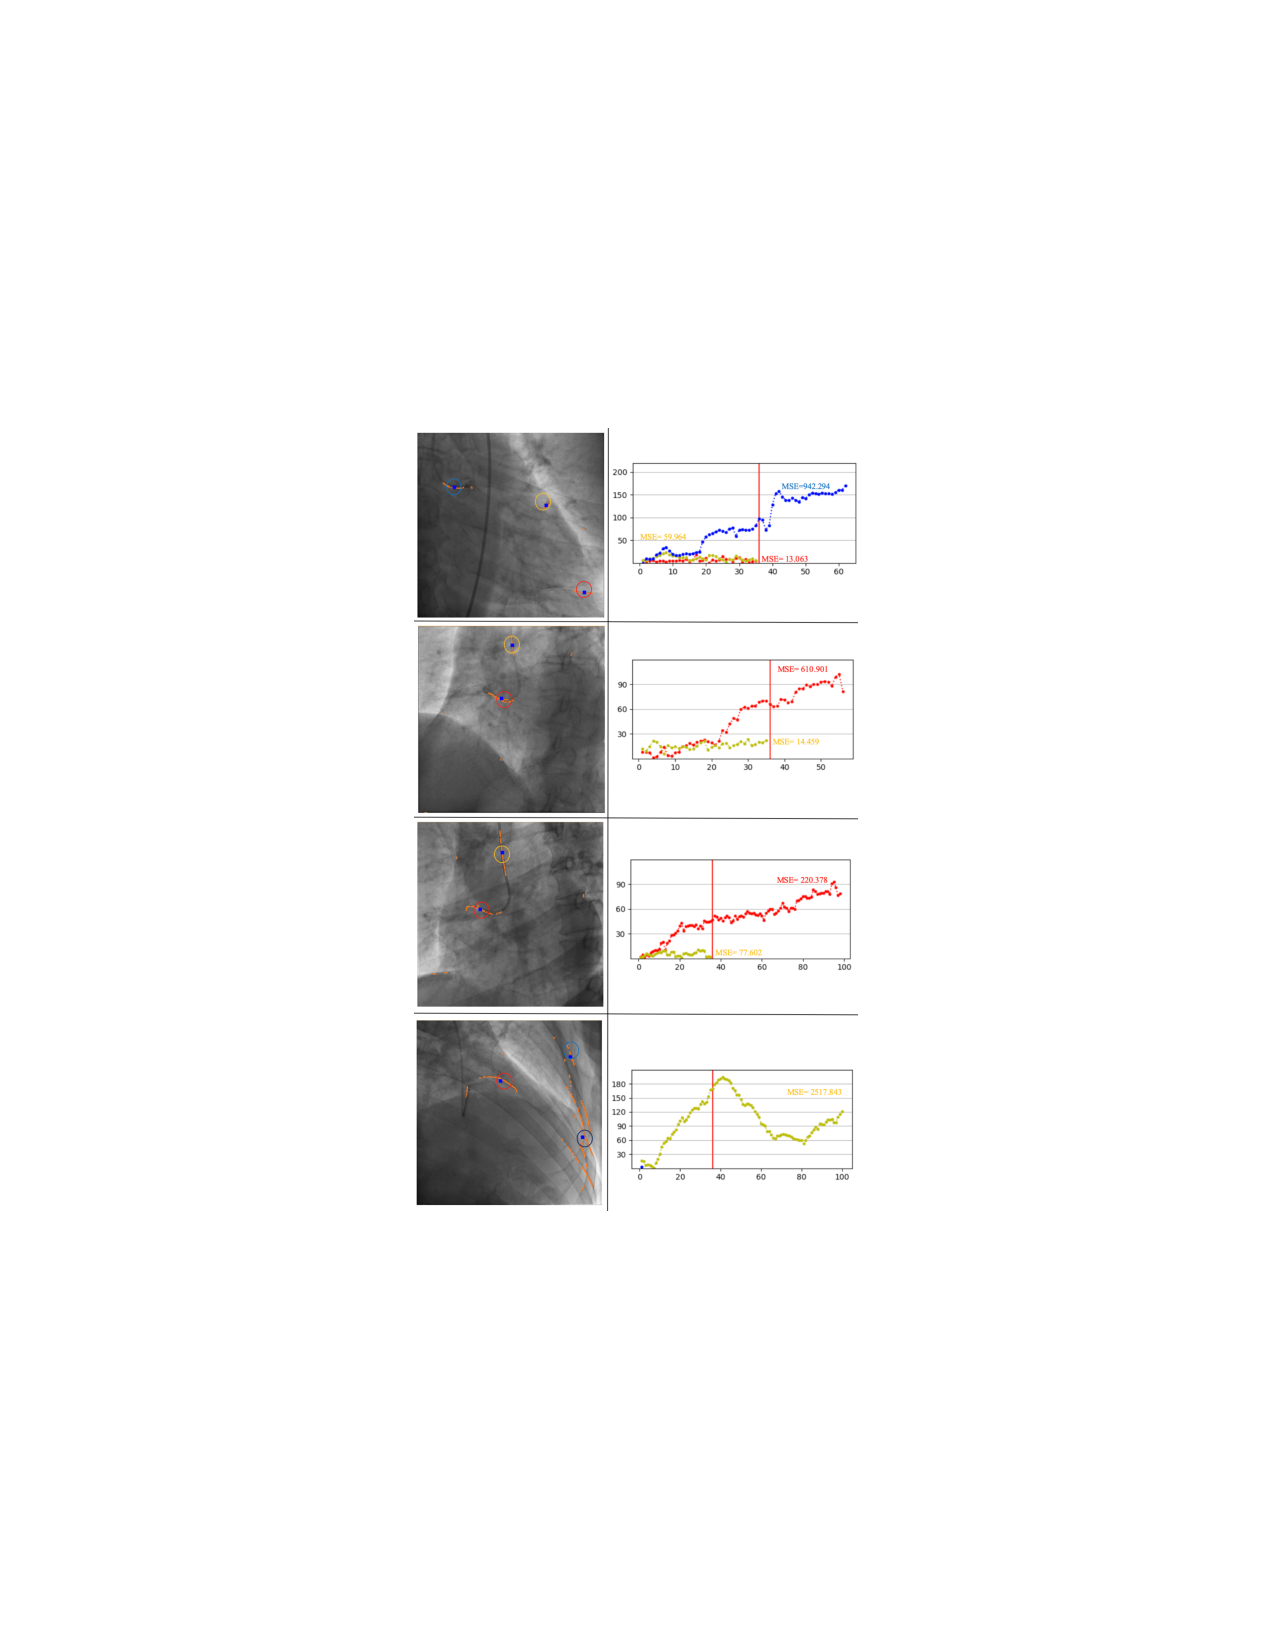
\includegraphics[width=3.5in]{figures/figure6}
		\caption{Guidewire Tip Recognition. The last case shows three candidates in the first frame however RuSio framework successfully recognized guidewire tip in second frame} 
	\label{fig:mcmthesis-logo} 
\end{figure}



\subsection{Guidewire Tip Recognition Procedure}
As we mentioned in the previous section, the first 36 frames are used to make the final decision of the guidewire tip from the underlying possibilities. In 9 x-ray videos experiment, the results have been shown a promising result of our guidewire tip recognition process which has a 100\% success rate. Also, in most cases the decision is making before the 36 frame.
\par
Four representative sequences are chosen to be shown the robust of the RuSio framework in guidewire tip recognition. The left section of Fig.5 showed all possible candidates(circle) and their gravity points(blue box) in each case when RuSio framework was initiated. Since there are always more than one candidates, RuSio framework will process parallel tracking that follows with a single target tracking strategy in order to distinguish guidewire tip through their motions. The right section of Fig.5 is Gravity Point Distance curve which records MSE for all candidates in each case. Also, X-axis represents the number of frames while Y-axis represents the distance of the gravity point between the current frame and first frame. After a short period tracking, RuSio framework successfully eliminates non-guidewire tip candidates. 

\begin{figure}[!htbp]
	\centering 
	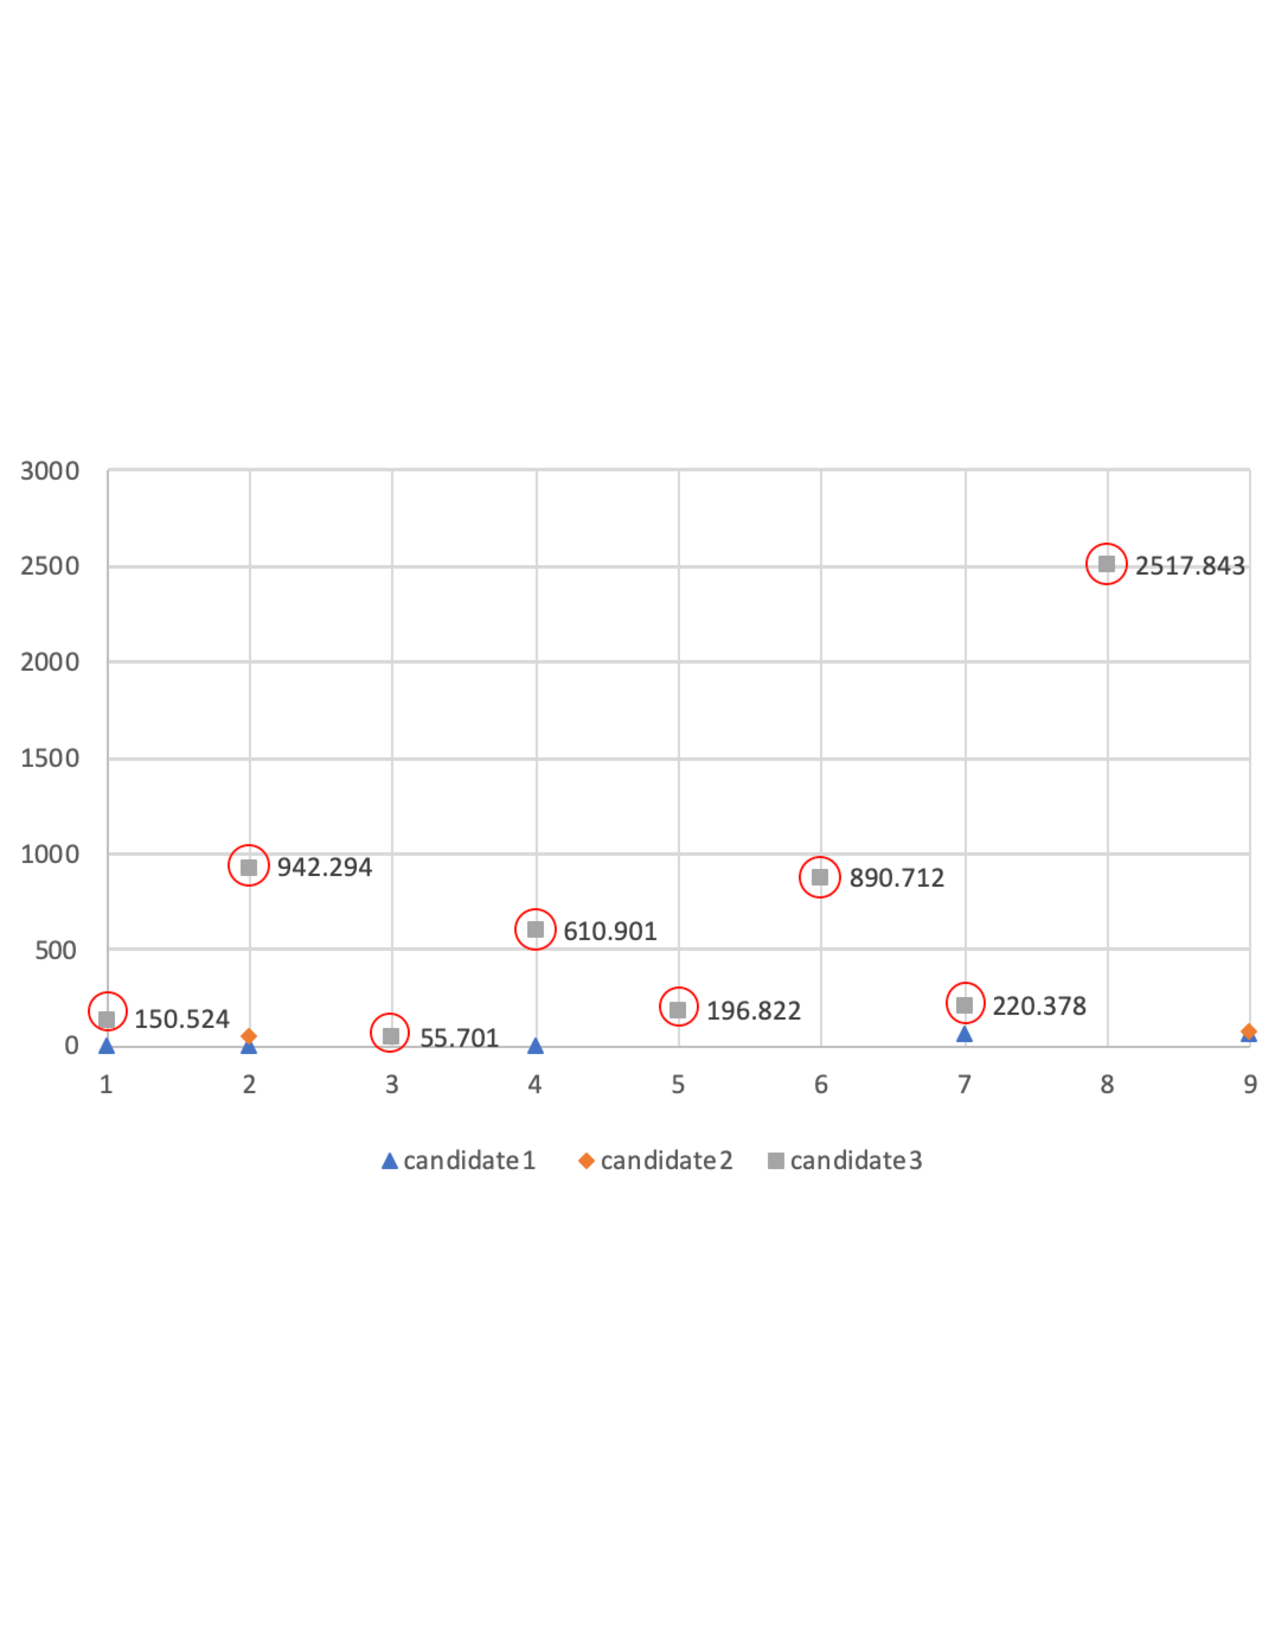
\includegraphics[width=3.5in]{figures/figure8}
		\caption{Guidewire tip recognition at the 36 frame for all 9 sequences. Grey square is guidewire tip with mean square error in fluoroscopic video sequences, RuSio framework successfully recognized guidewire tip at or before the 36 frame}  
	\label{fig:mcmthesis-logo} 
\end{figure}


\subsection{Guidewire Tip Tracking Performance}
Failure tracking frame defined as if any points in guidewire tip in current frame is beyond PGA. The tracking accuracy can be written as: 
\begin{equation}
TA= \frac{\#frames - \#failure}{\#frames}
\end{equation} 
The tracking accuracy of 9 video sequences is recorded in table I. 

In \cite{Jekel2018Similarity}, author clarified couple conceptions of methods which can measure the similarity between two curves, and also compared their performances. In order to show the RuSio framework’s segmentation accuracy more intuitively, Discrete Fr$\acute{e}$chet distance(DF) is used to show the similarity between tracking guidewire tip and the ground truth.\par
Fr$\acute{e}$chet distance measures the similarity between two curves which also considered the effection of location and ordering of the points along the curve \cite{Eiter1994Computing}. We will use discrete Fr$\acute{e}$chat distance here. In\cite{Eiter1994Computing} the discrete Fr$\acute{e}$chat distance defines a curve as a continuous mapping $f:[a,b] \rightarrow V$ where $a,b  \in  \mathbb{R}$ and a $\leq$ b. Also, (V,d) is a metric space. Given two curves, the discrete Fr$\acute{e}$chat distance is defined as 
\begin{equation}
\delta_F(f,g) =  inf_{\alpha,\beta}max_{t \in [0,1] }d(f(\alpha(t)),g(\beta(t)))\\
\end{equation}
where $\alpha, \beta$ are arbitrary continuous non-decreasing function from [0,1] to [a,b].\par

$F_{1}$ score is popular using for evaluation of tracking performance \cite{vandini2017robust}\cite{Peng2009Robust}\cite{6671560} .There are two factors which called missing and false tracking rate.
Missing tracking rate is the shortest distance from ground truth to tracked guidewire tip is greater than 3 pixels. 
False tracking rate is the shortest distance from tracked guidewire tip to the ground truth is greater than 3 pixels.
The $F_{1}$score combines two factors as in \cite{vandini2017robust}\cite{6671560}
\begin{equation}
F_{1} = 2*\frac{recall*precision}{recall+precision}
\end{equation}
where as 
\begin{equation}
recall = \frac{100-missing\%}{100}
\end{equation}
and
\begin{equation}
precision = \frac{100-false\%}{100}
\end{equation}

\begin{table}[!htb]
	\centering\input{../../../Downloads/math.log}

	\caption{Guidewire Tip Recognition Performance}
	\scalebox{0.9}{
	\begin{tabular}{cccccccc}
	\hline
	Sequence(\#)& MTR(\%)& FTR(\%)& F1score& MDF& SA & TA\\
	\hline
	2(137)&6.08&9.33&0.9227&1.98&89.78\%&96.35\%\\
	3(96)&9.42&14.7&0.8786&2.60&77.08\%&93.75\%\\
	4(108)&4.5&9.98&0.9268&1.75&97.22\%&90.74\%\\
	5(110)&7.74&5.87&0.9319&1.76&97.27\%&94.55\%\\
	6(73)&5.45&3.37&0.9558&1.92&95.89\%&94.52\%\\
	7(67)&2.06&6.95&0.9543&1.84&94.03\%&98.51\%\\
	8(196)&3.35&5.98&0.9562&1.87&93.37\%&98.98\%\\
	9(150)&0.85&2.23&0.9846&1.39&98\%&97.33\%\\
	10(53)&7.11&5.52&0.9368&1.81&92.45\%&96.31\%\\
	11(66)&8.07&3.73&0.9405&1.80&96.96\%&92.42\%\\
	\hline
	\end{tabular}}
\end{table}

\subsection{Case Exceptional Validation}
Even though the tracking algorithm operates with high stability in most cases, plenty of factors still could influence segmentation process such as the noise of background, the location of guidewire tip and varies angles of the X-ray machine or the guidewire tip hides in a set of guidewire-like objects and passes in front of catheters due to the non-rigid characteristic of the guidewire and the flexibility of the vessel. Segmenting the target structure turns out to be very difficult in special cases. 1).The guidewire tip instantly disappear due to low quality of video sequence.
2).The guidewire tip structure over-crossed or overlapped with the false curvilinear structure.
3).The guidewire tip curls up which make our framework extremely hard to define.

\begin{figure*}[!htb]
	\centering  
	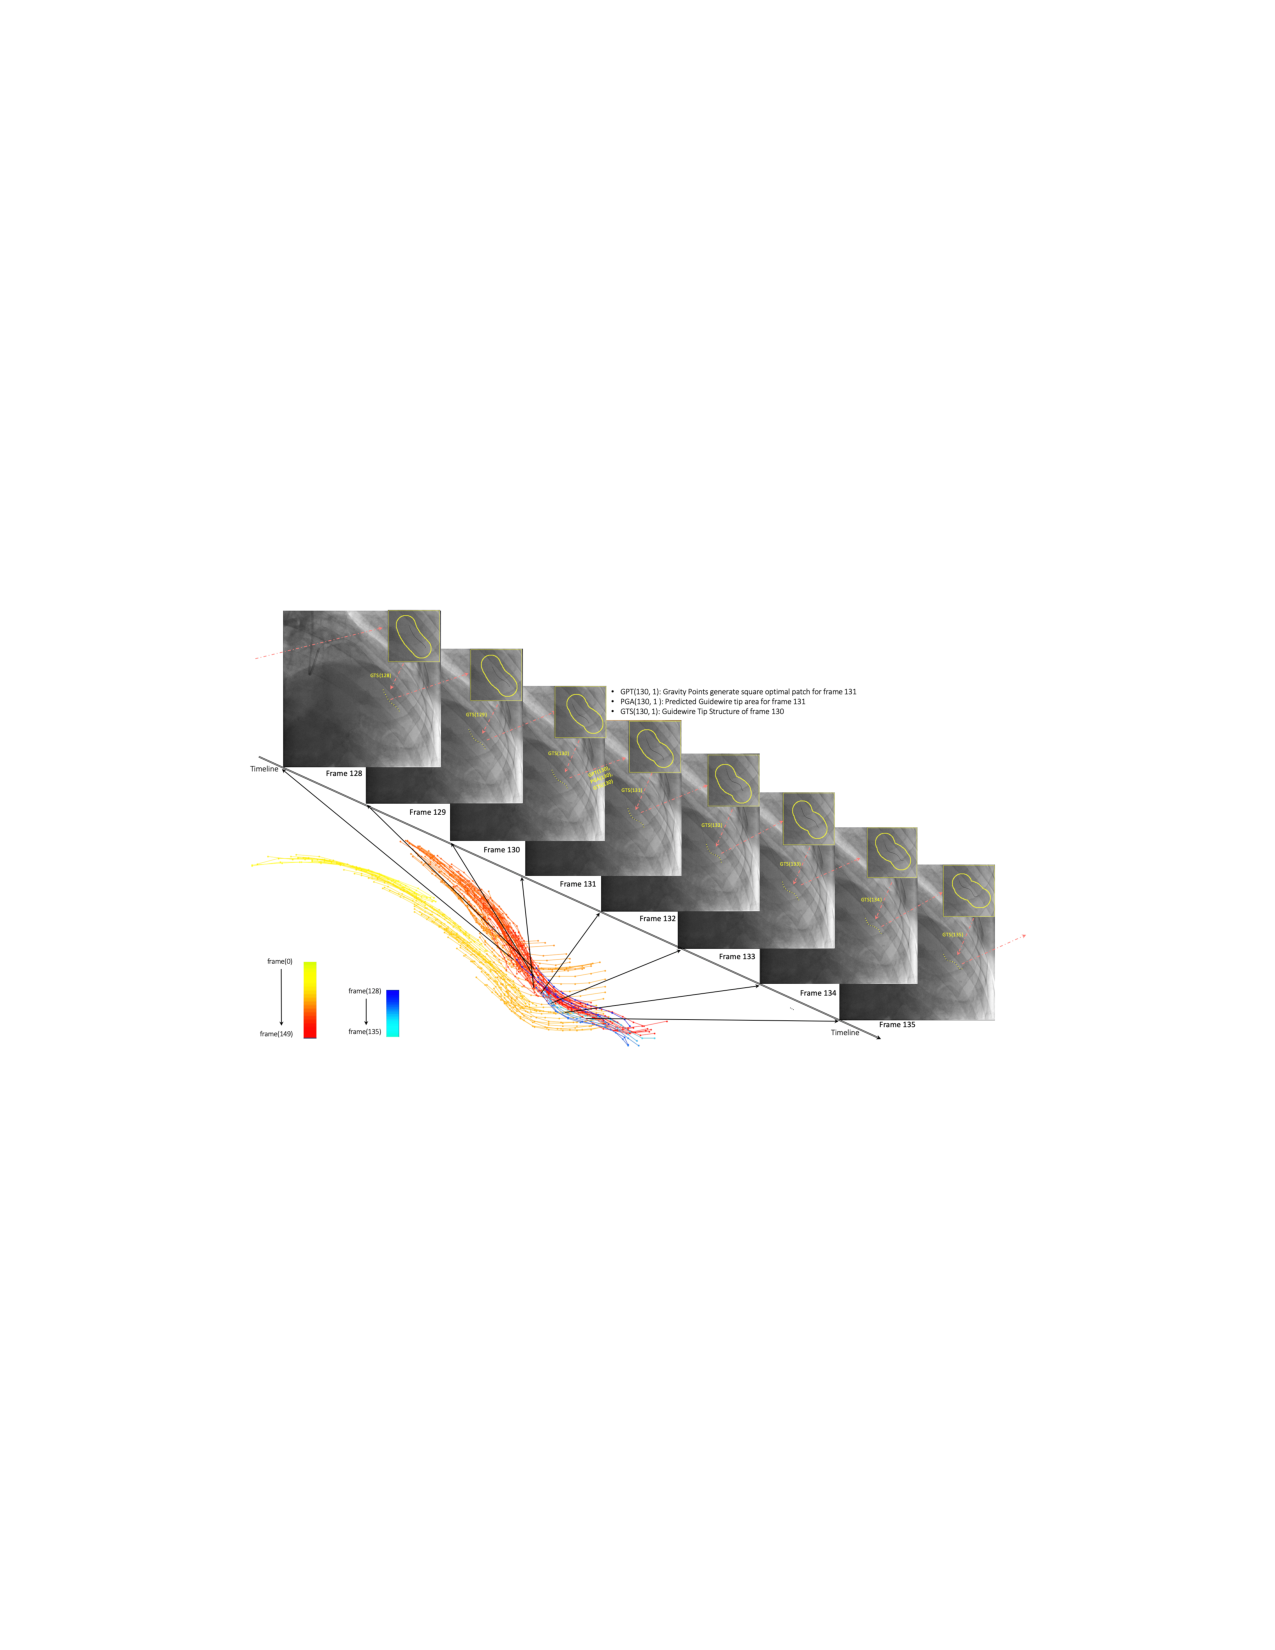
\includegraphics[width=7.1in]{figures/figure7}
		\caption{The segmentation collection of guidewire tip from RuSio framework in 8 consecutive frames from 128 to 135. The total frame of this sequence is 149.}  
	\label{fig:mcmthesis-logo} 
\end{figure*}

\begin{figure}[!htb]
	\centering  
	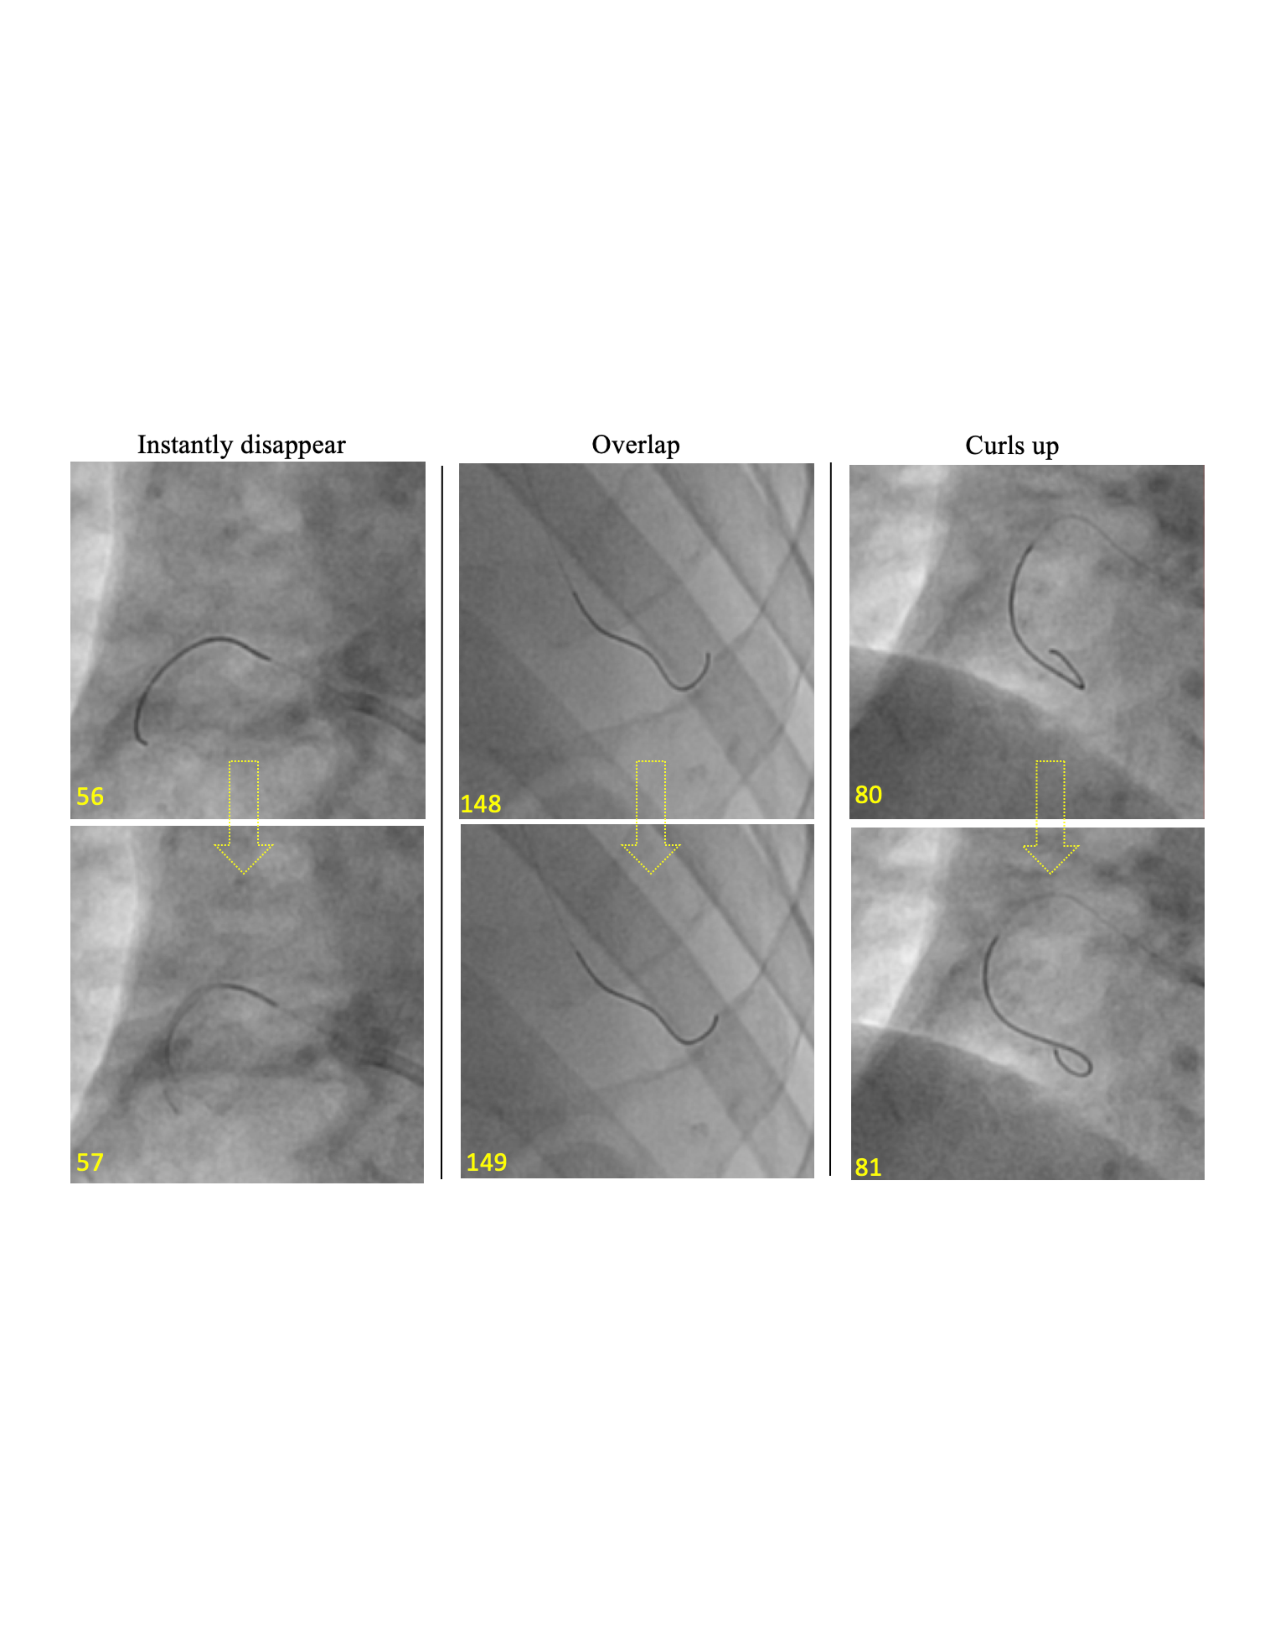
\includegraphics[width=3.5in]{figures/figure9}
		\caption{Exceptional cases} 
	\label{fig:mcmthesis-logo} 
\end{figure}




Overall, the proposed framework recognizes  the location of guidewire tip with 100\% accuracy and shows above 90\% in tracking the guidewire tip in most cases. In  \cite{vandini2017robust} the author mentioned the processing time of  SEGlets algorithm is 1-2 frames in 1 FPS without recognition of the guidewire tip. The processing time of RuSio framework in each frame included recognition and tracking is 1-2 frames in 1 FPS on average using Intel Core i7 (2.7GHz). Even though RuSio framework shows satisfying results in 9 fluoroscopic videos, the segmentation accuracy still can be improved.



\section{Discussion and Conclusion}
Guidewire tip's motion in X-ray fluoroscopic video during the cardiovascular intervention surgery is affected by many factors. For instance, moving curvilinear structures need to be separated to track the correct target. Guidewire tip, moreover, experiences abnormal elastic deformation because of its non-rigid feature. These factors make it more challenging to track the guidewire tip in 2D X-ray fluoroscopic video. This paper introduces a fully autonomous and robust tracking framework based on customized tracking strategy that is proven experimentally for its accuracy. As our framework is implemented in python with an average tracking performance of 0.6s per frame, Our team will move towards tracking performance acceleration to improve the integration into the PC Software of the C-arm X-Ray Machine where we can test our tracking framework in the clinical environment. 

As we have discussed earlier that the tracking of the guidewire tip in the fluoroscopic video is an important step to assist interventionist in making the correct decision during vascular intervention surgery. However, segmentation and shape of the guidewire tip are not sufficient in making the surgical procedure smarter for interventionists, since it only provides two-dimensional information which cannot be relied on for decision making. Deep logical development of artificial intelligent for interventional surgery is required. Our research team aims to improve the guidewire tip framework to provide more parameters such as heart rate and body temperature in the future. Besides, we should focus on the research problem on real-time co-registration between preoperative intervention planning and real-time fluoroscopic image to better understand where the guidewire is in a three-dimensional blood vessel. More importantly, with further research on the vascular interventional robot area, our tracking framework has a better application scenario to make the interventional robotic system more intelligent. In conclusion, our tracking framework improves the automation level of the computer-assisted vascular intervention.



% An example of a floating figure using the graphicx package.
% Note that \label must occur AFTER (or within) \caption.
% For figures, \caption should occur after the \includegraphics.
% Note that IEEEtran v1.7 and later has special internal code that
% is designed to preserve the operation of \label within \caption
% even when the captionsoff option is in effect. However, because
% of issues like this, it may be the safest practice to put all your
% \label just after \caption rather than within \caption{}.
%
% Reminder: the "draftcls" or "draftclsnofoot", not "draft", class
% option should be used if it is desired that the figures are to be
% displayed while in draft mode.
%
%\begin{figure}[!t]
%\centering
%\includegraphics[width=2.5in]{myfigure}
% where an .eps filename suffix will be assumed under latex, 
% and a .pdf suffix will be assumed for pdflatex; or what has been declared
% via \DeclareGraphicsExtensions.
%\caption{Simulation results for the network.}
%\label{fig_sim}
%\end{figure}

% Note that the IEEE typically puts floats only at the top, even when this
% results in a large percentage of a column being occupied by floats.


% An example of a double column floating figure using two subfigures.
% (The subfig.sty package must be loaded for this to work.)
% The subfigure \label commands are set within each subfloat command,
% and the \label for the overall figure must come after \caption.
% \hfil is used as a separator to get equal spacing.
% Watch out that the combined width of all the subfigures on a 
% line do not exceed the text width or a line break will occur.
%
%\begin{figure*}[!t]
%\centering
%\subfloat[Case I]{\includegraphics[width=2.5in]{box}%
%\label{fig_first_case}}
%\hfil
%\subfloat[Case II]{\includegraphics[width=2.5in]{box}%
%\label{fig_second_case}}
%\caption{Simulation results for the network.}
%\label{fig_sim}
%\end{figure*}
%
% Note that often IEEE papers with subfigures do not employ subfigure
% captions (using the optional argument to \subfloat[]), but instead will
% reference/describe all of them (a), (b), etc., within the main caption.
% Be aware that for subfig.sty to generate the (a), (b), etc., subfigure
% labels, the optional argument to \subfloat must be present. If a
% subcaption is not desired, just leave its contents blank,
% e.g., \subfloat[].


% An example of a floating table. Note that, for IEEE style tables, the
% \caption command should come BEFORE the table and, given that table
% captions serve much like titles, are usually capitalized except for words
% such as a, an, and, as, at, but, by, for, in, nor, of, on, or, the, to
% and up, which are usually not capitalized unless they are the first or
% last word of the caption. Table text will default to \footnotesize as
% the IEEE normally uses this smaller font for tables.
% The \label must come after \caption as always.
%
%\begin{table}[!t]
%% increase table row spacing, adjust to taste
%\renewcommand{\arraystretch}{1.3}
% if using array.sty, it might be a good idea to tweak the value of
% \extrarowheight as needed to properly center the text within the cells
%\caption{An Example of a Table}
%\label{table_example}
%\centering
%% Some packages, such as MDW tools, offer better commands for making tables
%% than the plain LaTeX2e tabular which is used here.
%\begin{tabular}{|c||c|}
%\hline
%One & Two\\
%\hline
%Three & Four\\
%\hline
%\end{tabular}
%\end{table}


% Note that the IEEE does not put floats in the very first column
% - or typically anywhere on the first page for that matter. Also,
% in-text middle ("here") positioning is typically not used, but it
% is allowed and encouraged for Computer Society conferences (but
% not Computer Society journals). Most IEEE journals/conferences use
% top floats exclusively. 
% Note that, LaTeX2e, unlike IEEE journals/conferences, places
% footnotes above bottom floats. This can be corrected via the
% \fnbelowfloat command of the stfloats package.

% if have a single appendix:
%\appendix[Proof of the Zonklar Equations]
% or
%\appendix  % for no appendix heading
% do not use \section anymore after \appendix, only \section*
% is possibly needed

% use appendices with more than one appendix
% then use \section to start each appendix
% you must declare a \section before using any
% \subsection or using \label (\appendices by itself
% starts a section numbered zero.)
%


%\appendix[Proof of the Zonklar Equations]



% you can choose not to have a title for an appendix
% if you want by leaving the argument blank


% use section* for acknowledgment
%\section*{Acknowledgment}


%The authors would like to thank...


% Can use something like this to put references on a page
% by themselves when using endfloat and the captionsoff option.
%\ifCLASSOPTIONcaptionsoff
%  \newpage
%\fi



% trigger a \newpage just before the given reference
% number - used to balance the columns on the last page
% adjust value as needed - may need to be readjusted if
% the document is modified later
%\IEEEtriggeratref{8}
% The "triggered" command can be changed if desired:
%\IEEEtriggercmd{\enlargethispage{-5in}}

% references section

% can use a bibliography generated by BibTeX as a .bbl file
% BibTeX documentation can be easily obtained at:
% http://mirror.ctan.org/biblio/bibtex/contrib/doc/
% The IEEEtran BibTeX style support page is at:
% http://www.michaelshell.org/tex/ieeetran/bibtex/

\bibliography{mybibliography}{}
\bibliographystyle{IEEEtran}
% argument is your BibTeX string definitions and bibliography database(s)
%\bibliography{IEEEabrv,../bib/paper}
%
% <OR> manually copy in the resultant .bbl file
% set second argument of \begin to the number of references
% (used to reserve space for the reference number labels box)
%\begin{thebibliography}{1}

%\bibitem{IEEEhowto:kopka}
%H.~Kopka and P.~W. Daly, \emph{A Guide to \LaTeX}, 3rd~ed.\hskip 1em plus
 % 0.5em minus 0.4em\relax Harlow, England: Addison-Wesley, 1999.

%\end{thebibliography}

% biography section
% 
% If you have an EPS/PDF photo (graphicx package needed) extra braces are
% needed around the contents of the optional argument to biography to prevent
% the LaTeX parser from getting confused when it sees the complicated
% \includegraphics command within an optional argument. (You could create
% your own custom macro containing the \includegraphics command to make things
% simpler here.)
%\begin{IEEEbiography}[{\includegraphics[width=1in,height=1.25in,clip,keepaspectratio]{mshell}}]{Michael Shell}
% or if you just want to reserve a space for a photo:

%\begin{IEEEbiography}{Michael Shell}
%Biography text here.
%\end{IEEEbiography}

% if you will not have a photo at all:
%\begin{IEEEbiographynophoto}{John Doe}
%Biography text here.
%\end{IEEEbiographynophoto}

% insert where needed to balance the two columns on the last page with
% biographies
%\newpage

%\begin{IEEEbiographynophoto}{Jane Doe}
%Biography text here.
%\end{IEEEbiographynophoto}

% You can push biographies down or up by placing
% a \vfill before or after them. The appropriate
% use of \vfill depends on what kind of text is
% on the last page and whether or not the columns
% are being equalized.

%\vfill

% Can be used to pull up biographies so that the bottom of the last one
% is flush with the other column.
%\enlargethispage{-5in}



% that's all folks
\end{document}


